\newif\ifdeDE\deDEfalse
\newif\ifenUS\enUSfalse



%%%% CHANGE OUTPUT LANGUAGE HERE %%%%
%% supported language codes:
\deDEtrue		% GERMAN
%\enUStrue		% ENGLISH




\documentclass{unisens}

\usepackage[latin1]{inputenc}
\usepackage[T1]{fontenc}

\ifdeDE
	\usepackage[ngerman]{babel}
\fi
\ifenUS
	\usepackage[english]{babel}
\fi


\usepackage{tabularx, varioref, mit_bib, graphicx}
\newcommand{\xmlattribute}[1]{\texttt{#1}}
\setcounter{secnumdepth}{0}

\begin{document}

\ifdeDE
\title{UnisensViewer\\[0.5em]\Large Anwender-Dokumentation}
\author{Malte Kirst, Marcus Warga}
\maketitle
\tableofcontents

	\section{Anwendungsgebiet}

Das Produkt dient zur vereinfachten Handhabung von Multisensor-Messdaten im Unisens-Format \cite{Kirst2008,Unisens2008} direkt nach
einer Datenaufzeichnung, sowie deren Visualisierung ("`Viewer"', "`Erster Angriff"'). Der
Arbeitsablauf soll durch softwareunterst�tzes Bearbeiten und Erstellen von Metadaten �ber
den Messdatensatz erleichtert werden. Die Metadaten werden hierbei im Unisens Format
gespeichert. Ebenso soll eine einfache Bearbeitung der Messdaten, wie z.\,B. das L�schen von
unbrauchbaren Signalteilen, erm�glicht werden. Weiterhin sollen in der Benutzeroberfl�che
f�r die wissenschaftliche Arbeit brauchbare Informationen �ber ausgew�hlte Messdaten,
sowie Annotationen angezeigt werden. Die Visualisierung von mehreren Messdatenstr�men
soll parallel und synchron sein, um Zusammenh�nge besser erfassen zu k�nnen.

 


	\section{Installation}

UnisensViewer ist eine Anwendung f�r Windows XP, Windows Vista und Windows 7. Sofern nicht vorhanden, ist das Microsoft .NET-Framework 4.0 oder h�her zu installieren. Auf manchen System ist es zus�tzlich erforderlich, das \textsl{Microsoft Visual C++ 2010 Redistributable Package} zu installieren. Beide Pakete sind auf der Microsoft Homepage verf�gbar \cite{Microsoft2010}.

Der Inhalt der ausgelieferten ZIP-Datei wird in ein beliebiges Verzeichnis entpackt. Die Datei \texttt{UnisensViewer.exe} ist sofort ausf�hrbar und startet die Anwendung.




	\section{Aufbau}

Der UnisensViewer (s. Abb. \ref{fig:viewer}) gliedert sich in drei Bereiche: Die Men�leiste (oben), die Seitenleiste am linken Rand und den Anzeigebereich auf der rechten Seite.

\begin{figure}[ht]
  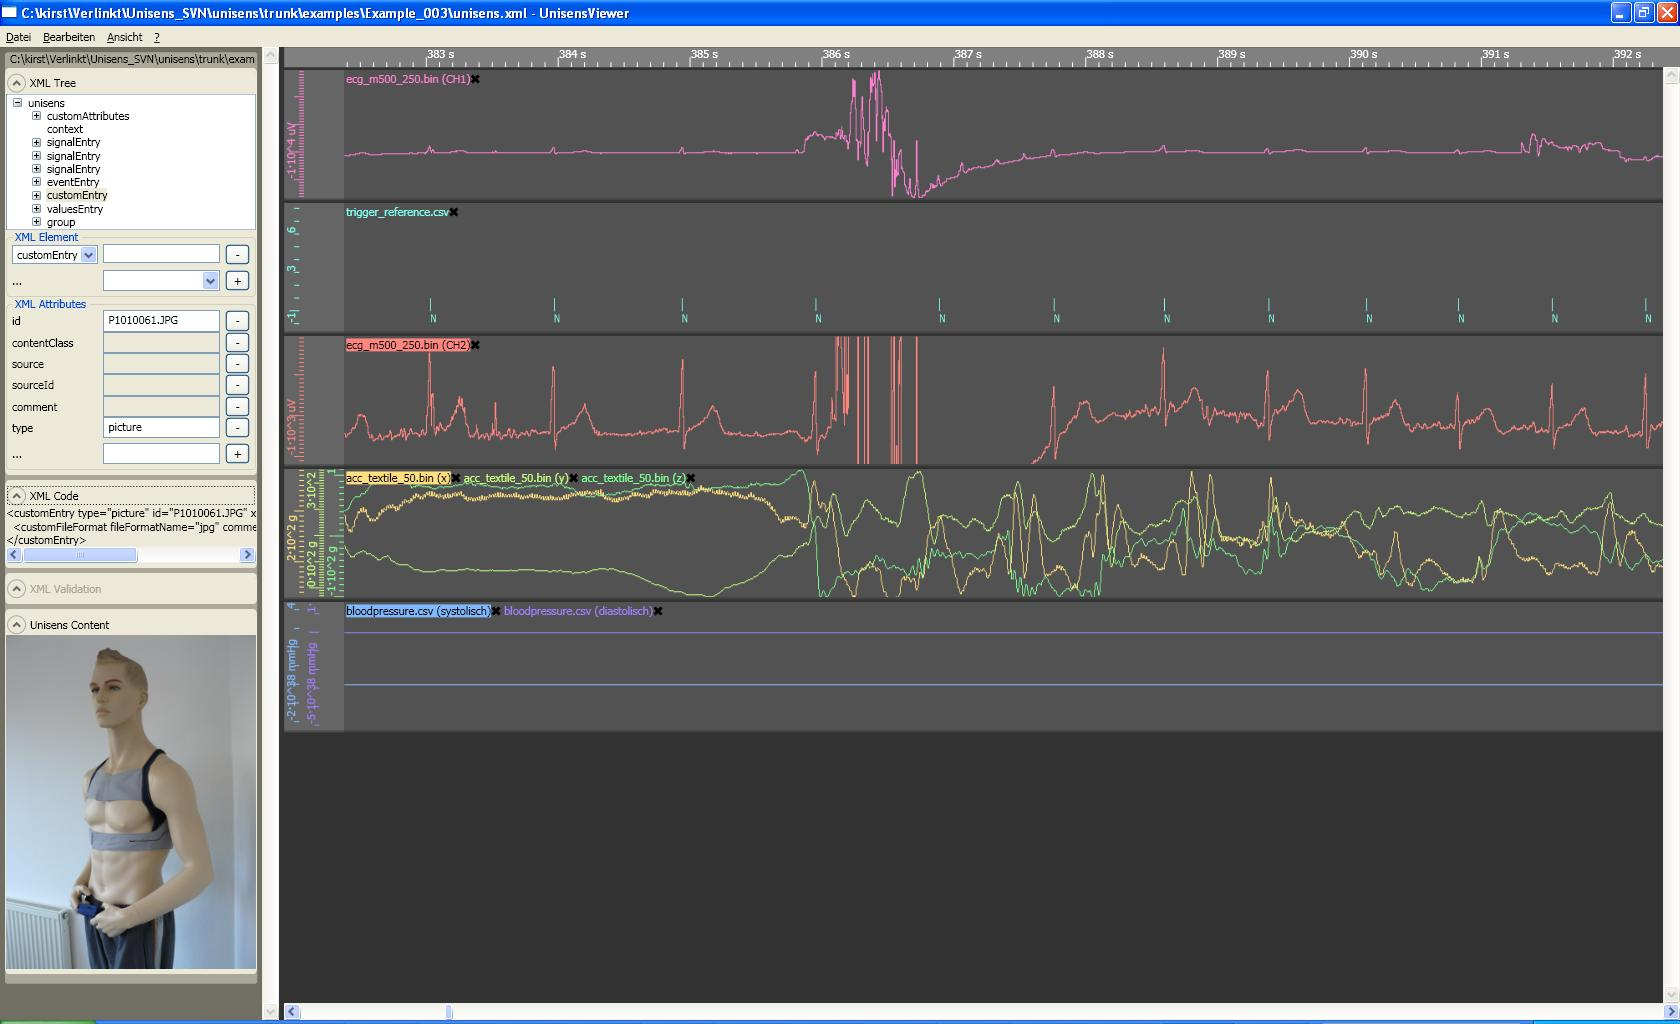
\includegraphics[width=\textwidth]{ressourcen/UnisensViewer.JPG}  	
	\caption{UnisensViewer: Am linken Rand ist die Seitenleiste, rechts der Anzeigebereich}
	\label{fig:viewer}
\end{figure}



		\subsection{Men�leiste}

Die Men�leiste am oberen Rand der Anwendung besteht aus folgenden Men�punkten:

\begin{description}
	\item[Datei] Men�punkte zum �ffnen und Speichern von Datens�tzen bzw. zum Erstellen eines neuen leeren Datensatzes.
	\item[Bearbeiten] Zur Zeit noch ohne Funktionalit�t.
	\item[Ansicht] Funktion zum automatischen Zoomen aller Y-Achsen.
	\item[?] Informationen �ber UnisensViewer.
\end{description}



		\subsection{Seitenleiste}
	
Die Seitenleiste enth�lt alle (Kontext-)Informationen aus der \texttt{unisens.xml}. Die Breite der Seitenleiste l�sst sich durch Ziehen mit der Maus ver�ndern. 

Innerhalb der Seitenleiste sind mehrere Fenster angeordnet. Im oberen Bereich befinden sich die Cursor-Informationen, hier werden Zeit- und Amplitudeninformationen der aktuellen Cursorposition angezeigt. Wird mit der Maus ein Signalbereich markiert, erscheinen weitere Informationen zum markierten Bereich.

Der XML-Baum (\textsl{XML Tree}) stellt die Metainformationen aus der \texttt{unisens.xml} in einer Baumstruktur dar. Man kann diesen Baum browsen, in dem man einzelne Elemente anklickt, aufklappt oder zuklappt. Zu einem markierten Element werden alle Attribute angezeigt.

Die Code-Ansicht (\textsl{XML Code}) zeigt den Bereich der \texttt{unisens.xml} an, der im XML-Baum markiert ist.

Die Validierungsansicht (\textsl{XML Validation}) zeigt die Informationen des integrierten XML-Validators. Sollte die \texttt{unisens.xml} nicht dem XSD (XML Schema Document) entsprechen, werden hier die Fehlermeldungen angezeigt.

In der Inhalts-Ansicht (\textsl{Unisens Content}) werden ausgew�hlte Inhalte des Datensatzes angezeigt. Dies kann zum Beispiel der Inhalt der \texttt{context.xml} (ebenfalls als XML-Baum mit Code und Validierung) oder ein CustomEntry.



		\subsection{Anzeigebereich}

Der Anzeigebereich zeigt Signale, Messwerte und Annotationen an. Mit Hilfe von Mausgesten kann gezoomt und gescrollt werden. Angezeigte Daten k�nnen per Drag \& Drop umsortiert und gestapelt werden.




	\section{Betrieb}

Die Datei \texttt{UnisensViewer.exe} ist sofort ausf�hrbar und startet die Anwendung. In diesem Abschnitt wird die Bedienung des Viewers beschrieben. Hauptmerkmale sind hier die Unterst�tzung von Mausgesten, Drag \& Drop und das Kontextmen�.



		\subsection{�ffnen von Datens�tzen}

Datens�tze k�nnen �ber den Datei-�ffnen-Dialog (\textsl{Datei} \textrightarrow\ \textsl{�ffnen...} oder \textsf{Strg} + \textsf{o}) oder �ber Drag \& Drop der Datei in den XML-Baum ge�ffnet werden. Anschlie�end erscheint im XML-Baum der Datensatz



		\subsection{Anzeigen von Signalen, Messwerten und Annotationen}

Um Signale, Messwerte und Annotationen anzuzeigen, wird das entsprechende Entry (SignalEntry, ValuesEntry oder EventEntry) aus dem XML-Baum in den Anzeigebereich gezogen. Jedes Entry kann nur einmal im Anzeigebereich angezeigt werden. Jedes angezeigte Element erh�lt ein Namensschild in der Form \textsl{EntryId (ChannelName)}. Die angezeigten Elemente k�nnen mit Drag \& Drop umsortiert, gestapelt oder auseinandergezogen werden. Die f�r Drag \& Drop sensitive Fl�che ist das Namensschild des entsprechenden Elements.



		\subsection{Benutzung des XML-Editors}

Der in die Seitenleiste integrierte XML-Editor ist zum Betrachten, Bearbeiten oder neu Anlegen der  \texttt{unisens.xml} bzw. der  \texttt{context.xml} zust�ndig. Schlagworte: XSD-Datei, Validierung, Attribute, Elemente
	
	
	
		\subsection{Anzeigen von CustomEntries}
	
Kontext-Informationen k�nnen im XML-Baum ausgew�hlt (\textsl{custom}) werden, sie werden dann im unteren Bereich (\textsl{Unisens Content}) in der Seitenleiste angezeigt. Bisher werden folgende Dateiformate unterst�tzt:

\begin{table}[ht]
	\caption{Unterst�tze Kontext-Informationen}
	\begin{tabularx}{\textwidth}{lX}
		\hline
		Dateiendung & Beschreibung \\
		\hline
		\hline
		JPG & Bildvorschau \\
		PNG & Bildvorschau \\
		\hline
	\end{tabularx}
	\label{tab:contentclass}
\end{table}
	\[
\]



		\subsection{Horizontales und vertikales Zoomen / Skalieren}
Zoomen und Skalieren der angezeigten Signale erfolgt �ber Mausgesten. Das horizontale Zoomen (Zeitachse) bezieht sich auf alle angezeigten Signale. Das vertikale Zoomen bzw. Skalieren bezieht sich auf alle ausgew�hlten Signale des aktuellen Stapels. Signale k�nnen �ber ihren Bezeichner ausgew�hlt werden.

\begin{description}
	\item[Horizontales Zoomen] Mittlere Maustaste + vertikale Mausgeste, Alt + mittlere Maustaste + vertikale Mausgeste oder
Alt + linke Maustaste + vertikale Mausgeste
	\item[Vertikales Zoomen]	Shift + mittlere Maustaste + horizontale Mausgeste
\end{description}



		\subsection{Verschieben und Scrollen}
Verschieben und Scrollen erfolgt �ber Mausgesten oder �ber den horizontalen Scrollbalken am unteren Rand der Anzeige. Das horizontale scrollen (Zeitachse) bezieht sich auf alle angezeigten Signale. Das vertikale scrollen bezieht sich auf alle ausgew�hlten Signale des aktuellen Stapels. Signale k�nnen �ber ihren Bezeichner ausgew�hlt werden.

\begin{description}
	\item[Horizontales scrollen]	Mittlere Maustaste + horizontale Mausgeste, Alt + mittlere Maustaste + horizontale Mausgeste, Alt + linke Maustaste + horizontale Mausgeste oder mit Scrollbalken
	\item[Vertikales scrollen]	Strg + mittlere Maustaste + vertikale Mausgeste
\end{description}

Durch gleichzeitiges Dr�cken von Strg + Shift k�nnen die Gesten f�r vertikales Scrollen und vertikales Zoomen kombiniert werden.


		\subsection{Automatisches Skalieren}
Die Signale k�nnen automatisch skaliert werden. Dazu w�hlt man im Kontextmen� unter automatisches skalieren (f�r den aktuellen Stapel oder f�r die ausgew�hlten Signale des aktuellen Stapels) oder im Hauptmen� - um alle angezeigten Signale zu skalieren - unter Ansicht, automatisch skalieren die gew�nschte Skalierungsfunktion aus. Folgende Skalierungsoptionen stehen zur Verf�gung:

\begin{description}
	\item[Signale individuell]	Die Signale werden so skaliert, dass jedes Signal f�r sich den Platz auf der Anzeige voll ausnutzt.
	\item[Nach Dateien gruppiert]	Die Signale werden vor der Skalierung gruppiert, alle Dateien aus einem Entry bilden dabei eine Gruppe. Diese Signale werden mit dem gleichen Faktor und um den gleichen Nullpunkt skaliert, so dass der Platz auf der Anzeige voll ausgenutzt wird.
	\item[Nach Einheiten gruppiert]	Die Signale werden vor der Skalierung gruppiert, alle Dateien mit gleicher physikalischer Einheit bilden dabei eine Gruppe. Diese Signale werden mit dem gleichen Faktor und um den gleichen Nullpunkt skaliert, so dass der Platz auf der Anzeige voll ausgenutzt wird.
\end{description}



	\subsection{Erstellen von neuen Datens�tzen}

Um einen neuen Unisens-Datensatz anzulegen, geht man im Men� auf \textsl{Datei} \textrightarrow\ \textsl{Neu}. Anschlie�end markiert man im XML-Baum das Element \texttt{Unisens} und f�llt im Editor die notwendigen Attribute aus. Den so erstellten Unisens-Datensatz speichert man am gew�nschten Ort.

Um dem Datensatz Entries hinzuzuf�gen, k�nnen diese per Drag \& Drop in den XML-Baum gezogen werden. Dabei ist darauf zu achten, dass sich die Daten im selben Ordner befinden, in dem auch die \texttt{unisens.xml}-Datei gespeichert wurde (ansonsten kann man den Datensatz sp�ter nicht �ffnen). Dabei werden \texttt{bin}-Dateien automatisch als SignalEntry und \texttt{csv}-Dateien automatisch als EventEntry angelegt.



	\section{Plug-Ins}
	
	\subsection{Installation}
	
UnisensViewer l�sst sich durch Plug-Ins erweitern. Die Installation von Plug-Ins erfolgt durch kopieren der Plug-In-Datei in den Ordner Plugins. Beim n�chsten Start des UnisensViewer erscheint das Plug-In im entsprechenden Men�. 



	\subsection{Aufruf}
	
Ein Plug-In kann -- je nach Art -- auf ein oder mehrere Entrys angewendet werden. 


	\section{Lizenz}

UnisensViewer ist eine Entwicklung des FZI Forschungszentrum Informatik. UnisensViewer wird kostenfrei und "`as-is"', ohne jegliche ausdr�ckliche oder stillschweigende Garantie, zur Verf�gung gestellt. In keinem Fall werden die Autoren f�r Sch�den, die aus der Nutzung dieser Software entstehen k�nnen, haftbar gemacht. 

Wenn Sie Unisens f�r wissenschaftliche Arbeiten nutzen, bitten wir Sie, in Ver�ffentlichungen auf das Unisens-Datenformat und die Unisens-Webseite \texttt{http://www.unisens.org} \cite{Unisens2008} hinzuweisen.

Die Unisens-Library und das Unisens-Interface stehen unter der GNU Lesser General Public License (LGPL). Der Lizenztext wird mit dem Code ausgeliefert und ist auf \cite{lgpl2008} einsehbar. Die Unisens-Library und das Unisens-Interface erhalten Sie auf der Unisens-Projektseite \texttt{http://www.unisens.org}.



%%%%%%%%%%%%%%%%%%%%%%%%%%%%%%%%%%%%%%%%%%%%%%%%%%%%%%%%%%%%%%%%%%%%%%%%%%%%%%%%%%%%
%
%  Literaturverzeichnis
%
%%%%%%%%%%%%%%%%%%%%%%%%%%%%%%%%%%%%%%%%%%%%%%%%%%%%%%%%%%%%%%%%%%%%%%%%%%%%%%%%%%%%


\bibliographystyle{mit_din}
\bibliography{Unisens}

%XML
%XSD
%CSV Format
%Floating Point Spec
%FAT16: http://de.wikipedia.org/wiki/File_Allocation_Table#FAT16
%WFDB Format: http://www.physionet.org/physiotools/wpg/wpg.htm
%\nocite{moody2008}


%%%%%%%%%%%%%%%%%%%%%%%%%%%%%%%%%%%%%%%%%%%%%%%%%%%%%%%%%%%%%%%%%%%%%%%%%%%%%%%%%%%%
%
%  Kontakt
%
%%%%%%%%%%%%%%%%%%%%%%%%%%%%%%%%%%%%%%%%%%%%%%%%%%%%%%%%%%%%%%%%%%%%%%%%%%%%%%%%%%%%

	\section*{Kontakt}

\paragraph{FZI Forschungszentrum Informatik} ~\\
Embedded Systems and Sensors Engineering (ESS)\\
Haid-und-Neu-Str. 10--14\\
76131 Karlsruhe\\[1ex]
Dipl.-Ing. Malte Kirst\\
kirst@fzi.de

\paragraph{Universit�t Karlsruhe} ~\\
Institut f�r Technik der Informationsverarbeitung (ITIV)\\
Engesserstr. 5\\
76131 Karlsruhe\\[1ex]
Dipl.-Ing. J�rg Ottenbacher\\
ottenbacher@itiv.uni-karlsruhe.de

\paragraph{http://www.unisens.org}

\fi

\ifenUS
\title{UnisensViewer\\[0.5em]\Large User Documentation}
\author{Kristina Schaaff, Malte Kirst, Marcus Warga}
\maketitle
\tableofcontents

	\section{Application Area}
	
UnisensViewer has been developed for easy handling of multi sensor data stored in the Unisens data format \cite{Kirst2008,Unisens2008} directly after the recording as well as for data visualization. The workflow is simplified by a software-based solution for editing and creating of meta data for data sets. This meta data is stored in the Unisens data format. Moreover, UnisensViewer allows to easily edit measurement data. Additionally, the user interface can be used to display information about selected measurement data as well as annotations. Visualization of multiple sensor data can be done synchronous and in parallel. 


	\section{Installation}

UnisensViewer is an application for Windows XP, Windows Vista and Windows 7. If not already installed, the .Net-Framework 4.0 or higher has to be installed. Some systems additionally require installation of \textsl{Microsoft Visual C++ 2010 Redistributable Package}. Both packages are available at the Microsoft homepage \cite{Microsoft2010}.

The content of the zip-file has to be unpacked to a folder of your choice. The file \texttt{UnisensViewer.exe} can be executed immediately and will start the UnisensViewer.  




	\section{Structure of UnisensViewer}

UnisensViewer (see Figure \ref{fig:viewer}) consists of three areas: the menu bar (upper side), the sidebar at the left side and the display area at the right side. 

\begin{figure}[ht]
  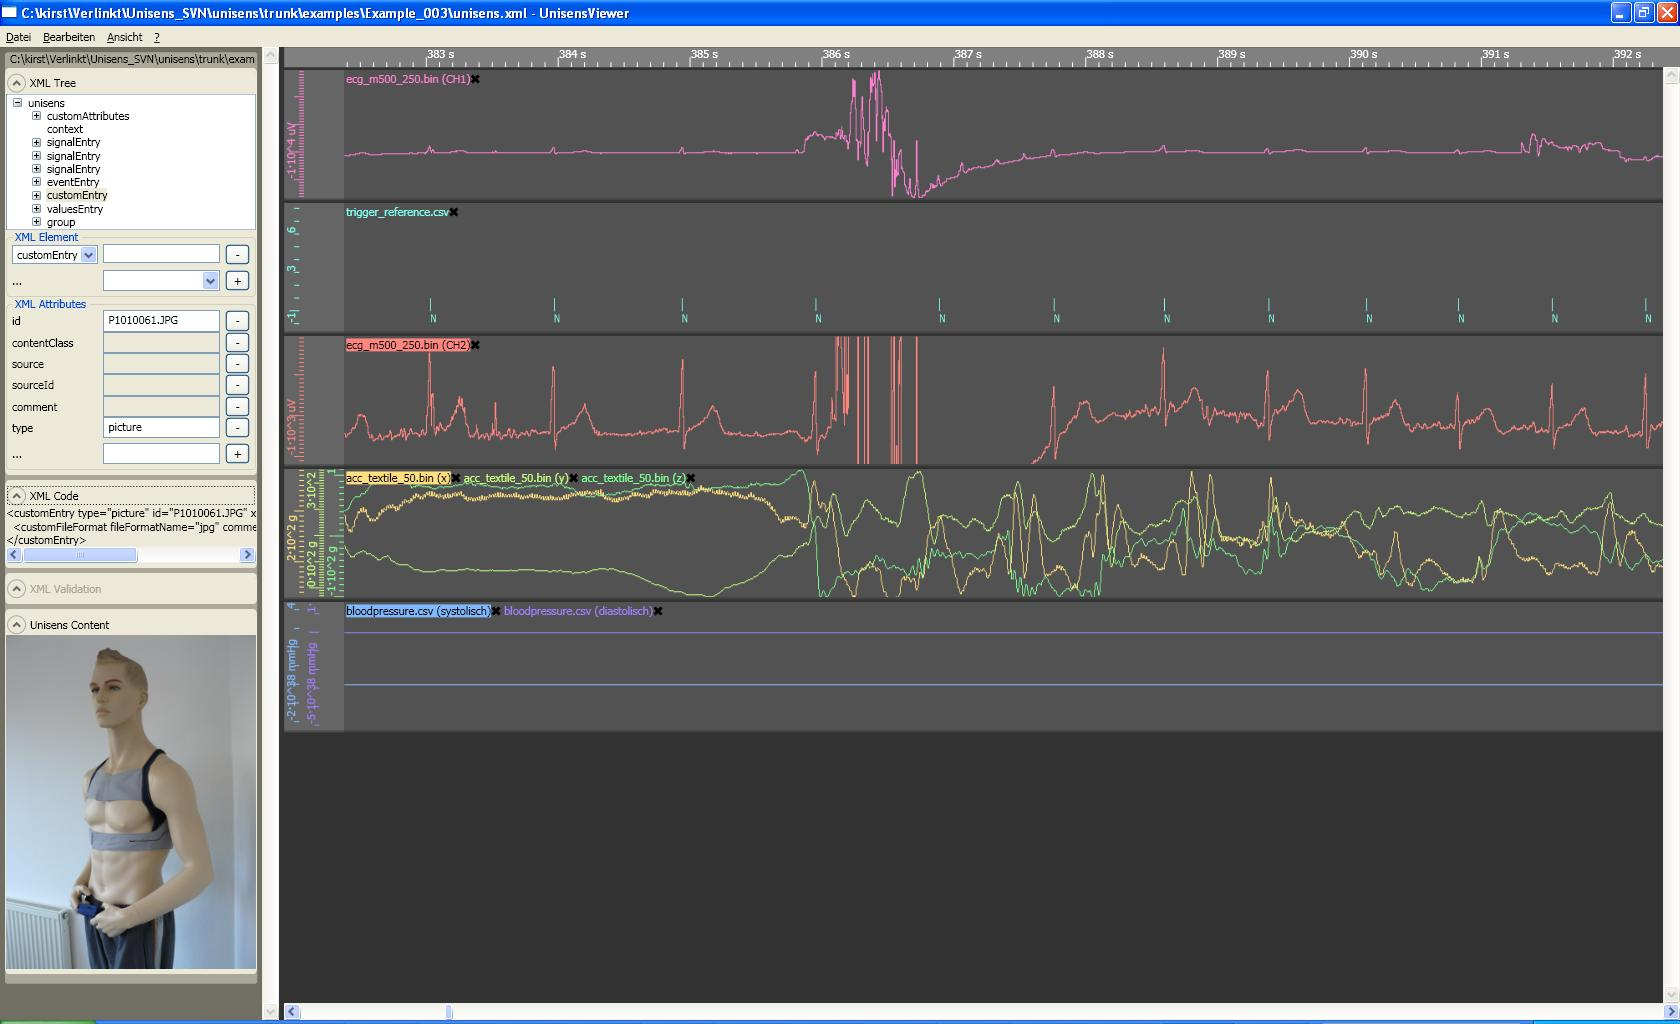
\includegraphics[width=\textwidth]{ressourcen/UnisensViewer.JPG}  	
	\caption{UnisensViewer: sidebar at the left side, display area on the right}
	\label{fig:viewer}
\end{figure}



		\subsection{Menu Bar}
		
The menu bar at the upper side of the window consists of the following items: 

\begin{description}
	\item[File] Open and save data sets and create new data sets
	\item[Edit] Not implemented yet
	\item[View] Functions for automatic zooming
	\item[Plug-ins] For installed plug-ins
	\item[?] Information about UnisensViewer
\end{description}



		\subsection{Sidebar}
	
The sidebar contains all (context) information from the \texttt{unisens.xml}. The width of the sidebar may be varied by dragging it with the mouse. 

Within the sidebar you will find various windows. The upper area contains cursor information displaying the time- and amplitude information of the current cursor position. If a signal part is marked with the mouse, further information about the marked area appears. 

The XML tree displays the meta information from the \texttt{unisens.xml} in a tree structure. It is possible to browse this tree by klicking at the elements to fold or unfold the elements. For the selected element all corresponding attributes are shown at the sidebar. 


The code view (\textsl{XML Code}) shows the area of the \texttt{unisens.xml} which is marked in the XML tree. 

The validation view  (\textsl{XML Validation}) shows the information of the integrated XML validator. If the \texttt{unisens.xml} is not conform to the associated XSD (XML Schema Document), errors are shown in this view. 

The content view (\textsl{Unisens Content}) contains selected contents of a data set. This can for instance be the content of the \texttt{context.xml} or a CustomEntry. 



		\subsection{Display Area}
		
The display area shows signals, measurement values and annotations. Mouse gestures can be used for zooming and scrolling. The data displayed can be moved and / or stacked by drop \& drag. 


	\section{Using the UnisensViewer}

The file \texttt{UnisensViewer.exe} can be executed immediately and will start the program. This section describes the usage of the Viewer. Main features are the support of mouse gestures, drag \& drop and the context menu.


		\subsection{Opening Data Files}
		
Data files can be opened using the open file dialog (\textsl{File} \textrightarrow\ \textsl{Open...} or \textsf{Ctrl} + \textsf{o}) or by drop \& drag of the file into the XML tree. Subsequently, the data set will appear in the XML tree. 


		\subsection{Displaying Signals, Measured Data and Annotations}

To display signals, measured data and annotations, the corresponding entry (SignalEntry, ValuesEntry or EventEntry) has to be dragged from the XML tree to the display area. Each entry can only be displayed once in the display area. All elements include a name tag in the format \textsl{EntryId (ChannelName)}. The displayed elements can be resorted by drag \& drop, stapled, or unstapled. The area which is sensitive for drag \& drop is the name tag of the corresponding element. 


		\subsection{Using the XML Editor}

The XML editor which is integrated in the sidebar is responsible to view, edit or create the files \texttt{unisens.xml} and \texttt{context.xml}. 
	
	
	
		\subsection{Display of CustomEntries}
		
Context information can be chosen from the XML tree, it is displayed in the lower area (\textsl{Unisens Content}) of the sidebar. Until now, the following data formats are supported: 
	
\begin{table}[ht]
	\caption{Supported context information}
	\begin{tabularx}{\textwidth}{lX}
		\hline
		file extension & description \\
		\hline
		\hline
		JPG & picture preview \\
		PNG & picture preview \\
		\hline
	\end{tabularx}
	\label{tab:contentclass}
\end{table}
	\[
\]



		\subsection{Horizontal and Vertical Zooming / Scaling}
Zooming and scaling of the displayed signals is done by mouse gestures. Horizontal zooming (time axis) includes all displayed signals. Vertical zooming / scaling includes all chosen signals of the current stack. Signals can be chosen by klicking on the name tag. 

\begin{description}
	\item[Horizontal zooming] middle mouse button + vertical mouse gesture, Alt + middle mouse button + vertical mouse gesture or Alt + left mouse button + vertical mouse gesture
 	\item[Vertical zooming] shift + middle mouse button + horizontal mouse gesture
\end{description}



		\subsection{Moving and Scrolling}
Moving and scrolling of signals is done by mouse gestures or by the horizontal scroll bar at the lower side of the display. Horizontal scrolling (time axis) includes all displayed signals. Vertical scrolling refers to all selected signals of the current stack. Signals can be chosen by their name tag. 


\begin{description}
	\item[Horizontal scrolling] middle mouse button + horizontal mouse gesture, Alt + middle mouse button + horizontal mouse gesture, Alt + left mouse button + horizontal mouse gesture, or by using the scroll bar
	\item[Vertical scrolling] Ctrl + middle mouse button + vertical mouse gesture
\end{description}

By pressing Ctrl + Shift at the same time, gestures for vertical scrolling and vertical zooming can be combined. 




		\subsection{Automatic Scaling}
		
Signals can be scaled automatically. For automatic scaling \textsl{Auto scale} has to be selected from the context menu (for the current stack or the selected signals of the current stack). To scale all displayed signals, select \textsl{View} \textrightarrow\ \textsl{Auto scale} from the menu bar and select the preferred scaling function. The following scaling options are supported: 


\begin{description}
	\item[Distinct signals] Signals are scaled such that each signal fully uses the available space. 
	\item[Grouped by files] Signals are grouped before scaling, all files belonging to one entry belong to one group. These signals are scaled around zero with the same factor such that the space at the display is fully used. 
	\item[Grouped by units] Before scaling, signals are grouped, all data files with the same physical dimension belong to the same group. These signals are scaled with the same factor around zero such that the display space is fully used. 
\end{description}



	\subsection{Create New Data Sets}
	
To create a new data set, select \textsl{File} \textrightarrow\ \textsl{New} from the menu or press Ctrl + N. Subsequently, the elements from tre XML tree have to be selected. Next the required attributes can be filled in using the editor. The Unisens data set can then be stored at a folder of your choice. 

Entries can be added to the data set by putting them per drag \& drop to the XML tree. The files have to be locaed in the same folder like the \texttt{unisens.xml} (otherwise data set cannot be opened later). \texttt{bin} files are automatically added as a SignalEntry while \texttt{csv} files are added as EventEntry. 


	\section{Plug-Ins}
	
	\subsection{Installation}
	
It is possible to extend the UnisensViewer by plug-ins. The installation of plug-ins is done by copying the plug-in file into the folder \textsl{Plugins}. After the next start fo the UnisensViewer, the plug-in appears in the corresponding menu. 



	\subsection{Using Plug-Ins}
	
A plug in can - depending on the kind of the plugin - be used for single or multiple entries. 


	\section{License}

UnisensViewer is a development of FZI Forschungszentrum Informatik. The software is provided "as is", without warranty of any kind, express or implied, including but not limited to the warranties of merchantability, fitness for a particular purpose and noninfringement. In no event shall the consortium be liable for any claim, damages or other liability, whether in an action of contract, tort or otherwise, arising from, out of or in connection with the software or the use or other dealings in the software.

If you use Unisens for scientific research, please refer to the Unisens data format and the Unisens homepage  \texttt{http://www.unisens.org} \cite{Unisens2008} in your publications. 

The Unisens library and the Unisens interface are licensed under GNU Lesser General Public License (LGPL). The license text is delivered together with the code and can be found at \cite{lgpl2008}. You can get the Unisens libary and the Unisens interface at the Unisens project homepage \texttt{http://www.unisens.org}.



%%%%%%%%%%%%%%%%%%%%%%%%%%%%%%%%%%%%%%%%%%%%%%%%%%%%%%%%%%%%%%%%%%%%%%%%%%%%%%%%%%%%
%
%  Literaturverzeichnis
%
%%%%%%%%%%%%%%%%%%%%%%%%%%%%%%%%%%%%%%%%%%%%%%%%%%%%%%%%%%%%%%%%%%%%%%%%%%%%%%%%%%%%


\bibliographystyle{mit_din}
\bibliography{Unisens}

%XML
%XSD
%CSV Format
%Floating Point Spec
%FAT16: http://de.wikipedia.org/wiki/File_Allocation_Table#FAT16
%WFDB Format: http://www.physionet.org/physiotools/wpg/wpg.htm
%\nocite{moody2008}


%%%%%%%%%%%%%%%%%%%%%%%%%%%%%%%%%%%%%%%%%%%%%%%%%%%%%%%%%%%%%%%%%%%%%%%%%%%%%%%%%%%%
%
%  Kontakt
%
%%%%%%%%%%%%%%%%%%%%%%%%%%%%%%%%%%%%%%%%%%%%%%%%%%%%%%%%%%%%%%%%%%%%%%%%%%%%%%%%%%%%

	\section*{Contact}

\paragraph{FZI Forschungszentrum Informatik} ~\\
Embedded Systems and Sensors Engineering (ESS)\\
Haid-und-Neu-Str. 10--14\\
76131 Karlsruhe\\
Germany\\[1ex]
Dipl.-Ing. Malte Kirst\\
kirst@fzi.de

\paragraph{Universit�t Karlsruhe} ~\\
Institut f�r Technik der Informationsverarbeitung (ITIV)\\
Engesserstr. 5\\
76131 Karlsruhe\\
Germany\\[1ex]
Dipl.-Ing. J�rg Ottenbacher\\
ottenbacher@itiv.uni-karlsruhe.de

\paragraph{http://www.unisens.org}

\fi



\end{document}

